\section{Sky and Compass Model}
\label{sec:sky}
\subsection{Radiative transfer}
The earlier studies used the single scattering Rayleigh law $d = d_{\max}\sin^2\theta_s/(1+\cos^2\theta_s)$ for the zenith DoP, with $d_{\max}=0.6$ \cite{horvath, liang}. Study~3 replaces it with a vector Monte Carlo radiative transfer model (SIMULATED) of a plane parallel atmosphere: Rayleigh scattering (optical depth 0.17, about 470 nm), one aerosol type with a Henyey Greenstein phase function ($g=0.7$, single scattering albedo 0.92) and a Rayleigh shaped linear polarisation of maximum 0.2, a Lambertian depolarising ground (albedo 0.3) and full multiple scattering \cite{pust, zeng08}. Stokes vectors are carried with explicit reference frames and the radiance toward the zenith and toward a ring of twelve points at 60 degrees elevation is estimated by the local estimate method. In the single scattering limit the code reproduces the analytic Rayleigh DoP and the zenith angle of polarisation to within \sSSerr{} (unit tests). The aerosol phase matrix is a simplification, not a Mie computation; its parameters and the albedo are varied in a sensitivity run. The aerosol optical depth comes from the NASA POWER monthly climatology at 550 nm for Abu Dhabi (annual mean \sAODann{}, June \sAODjun{}, July \sAODjul{}) \cite{power}; AERONET was not reachable from the analysis environment.

\subsection{Validation against measurements}
Two measurements constrain the model. In the Tunisian desert, Horv\'ath and Wehner measured a zenith DoP of 24 to 30 percent at a solar elevation of 35 degrees and about 8 percent at 70 degrees \cite{horvath}. The model gives \sRTthirtyfiveLow{} at that first geometry for the lowest aerosol (AOD 0.15) and \sRTthirtyfiveMean{} at the Abu Dhabi mean, and \sRTseventyLow{} at 70 degrees; the near sun value of 8 percent exceeds even single scattering Rayleigh (6.2 percent), so we treat it as unexplained. Second, we analysed one day (29 July 2022) of the open Marseille full sky polarisation images of Poughon \emph{et al.} \cite{poughon24} (MEASURED, CC BY-SA 4.0): \sMeasN{} daylight images, zenith patch of 80 by 80 pixels. The zenith DoP follows $\sin^2\theta_s$ closely (correlation \sMeasCorr{}), and on images labelled clear the Rayleigh law fits with $d_{\max} = \sMeasDmax{}$, essentially the value assumed in the earlier studies, while the radiative transfer model at low aerosol lies about 15 percent lower at solar zenith 50 to 70 degrees. The measured angle of polarisation follows the solar meridian with a median absolute residual of \sMeasAopMad{} degrees after fitting the unknown camera orientation; this residual includes the camera tilt and centring and is not used to refit the sensor. We therefore keep the radiative transfer table as the primary (conservative) model and add a measured anchored table, with the clear sky law from the Marseille fit and aerosol and dust attenuation from radiative transfer, as a secondary model. No sign flip of the zenith polarisation (a neutral point) appears in any table cell with a usable DoP.

\subsection{Blind window, geometry and latitude}
With the frozen sensor law $\sigma_\alpha^2 = \sigma_f^2 + (c/d)^2$ ($\sigma_f = 0.5^\circ$, $c = 0.05^\circ$), the zenith compass noise on 21 June in Abu Dhabi exceeds 10 degrees for \sWinRT{} minutes under radiative transfer with the June aerosol (\sWinRTlo{} to \sWinRThi{} minutes for half to one and a half times that aerosol) and for \sWinAnch{} minutes with the measured anchored table, against 64 minutes in Study~2. The window lies only in May, June and July on the 21st of each month examined. Fig.~\ref{fig:s3sky} shows the model and the day.

Heading information from a set of sky points follows from the Cram\'er Rao bound $\sigma_\psi^{-2} = \sum_k (\partial\alpha_k/\partial\psi)^2/\sigma_{\alpha,k}^2$, with the derivative of each point's angle of polarisation from the scattering plane geometry and its noise from the radiative transfer DoP. A Monte Carlo least squares estimator matches the bound to within \sCRBdev{} percent from 3 to 40 degrees solar zenith. When the sun is exactly at the zenith the pattern is rotationally symmetric and no polarisation geometry can give heading; away from it a ring of points at 60 degrees elevation gains information much faster than the zenith point, because the off zenith angles rotate with the sun azimuth at first order while the zenith DoP grows only at second order. Adding the ring cuts the 21 June window to \sWinRing{} minutes (radiative transfer) and \sWinRingAnch{} minutes (anchored); a sun direction sensor (0.5 degrees, ASSUMED) has a window of \sWinSun{} minutes. Only a non celestial cue such as a magnetometer (ASSUMED error model) removes the window entirely; no sky geometry does. Under radiative transfer a zenith compass window occurs at every latitude between about \sLatMax{} degrees south and north, which includes the Sahara, the Arabian deserts, the Thar, the Kalahari, the Namib, the Atacama and the Australian deserts.


\begin{figure*}[t]
\centering
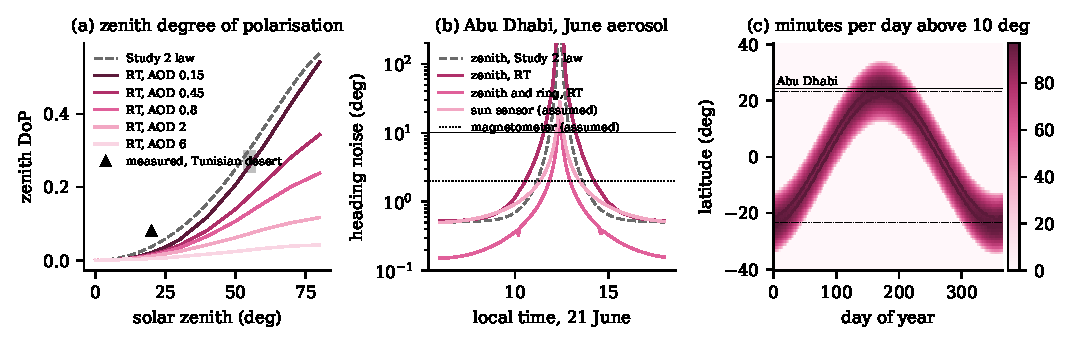
\includegraphics[width=\textwidth]{figs/fig_e03_sky.pdf}
\caption{Study 3 sky model (SIMULATED, with MEASURED reference points). (a) Zenith DoP against solar zenith for the radiative transfer model at five aerosol optical depths, the earlier single scattering law and the measured desert values \cite{horvath} (grey box and triangle). (b) Heading noise on 21 June in Abu Dhabi with the June aerosol for the zenith point, the zenith plus ring geometry and a sun sensor; dotted line, the assumed magnetometer. (c) Minutes per day with zenith compass noise above 10 degrees by latitude and day of year (aerosol 0.3).}
\label{fig:s3sky}
\end{figure*}

\subsection{Compass error model}
Study~3 adds, on top of the point noise: a heading bias (initial 1 degree, random walk 0.01 degrees per root second); the exact tilt error of a compass that assumes it is level, from the sun geometry and the platform roll and pitch (a Gauss Markov process of 2 degrees and 20 s on the development split; the protocol took roll and pitch from the rendered poses on the confirmation split, which turned out to be level, so tilt enters there through a sensitivity run); broken cloud with the POWER monthly cloud amount as the probability of a cloudy scenario; and, in the primary analysis, a near ground dust layer whose optical depth $3.912H/V$ ($H = 100$ m, assumed) follows the image visibility $V$ of each degradation level, so that a 20 m visibility image comes with a dust sky. The filter's noise estimate uses only the measured zenith DoP and the frozen law, so it no longer matches the simulated error; this removes the circularity of the earlier B3 result.
